\documentclass[12pt]{article}
\usepackage{tabularx} % extra features for tabular environment
\usepackage{amsmath}  % improve math presentation
\usepackage{graphicx} % takes care of graphic including machinery
\usepackage[margin=1in,letterpaper]{geometry} % decreases margins
\usepackage{cite} % takes care of citations
\usepackage[final]{hyperref} % adds hyper links inside the generated pdf file
\usepackage{mathtools}
\usepackage[utf8]{inputenc}

\usepackage{listings}
\usepackage{xcolor}
\usepackage{float}
% \usepackage[demo]{graphicx}
\usepackage{caption}
\usepackage{subcaption}

%New colors defined below
\definecolor{codegreen}{rgb}{0,0.6,0}
\definecolor{codegray}{rgb}{0.5,0.5,0.5}
\definecolor{codepurple}{rgb}{0.58,0,0.82}
\definecolor{backcolour}{rgb}{0.95,0.95,0.92}

%Code listing style named "mystyle"
\lstdefinestyle{mystyle}{
  backgroundcolor=\color{backcolour},   commentstyle=\color{codegreen},
  keywordstyle=\color{magenta},
  numberstyle=\tiny\color{codegray},
  stringstyle=\color{codepurple},
  basicstyle=\ttfamily\footnotesize,
  breakatwhitespace=false,         
  breaklines=true,                 
  captionpos=b,                    
  keepspaces=true,                 
  numbers=left,                    
  numbersep=5pt,                  
  showspaces=false,                
  showstringspaces=false,
  showtabs=false,                  
  tabsize=2
}

%"mystyle" code listing set
\lstset{style=mystyle}


\DeclarePairedDelimiter\floor{\lfloor}{\rfloor}

\hypersetup{
	colorlinks=true,       % false: boxed links; true: colored links
	linkcolor=blue,        % color of internal links
	citecolor=blue,        % color of links to bibliography
	filecolor=magenta,     % color of file links
	urlcolor=blue         
}
\usepackage{blindtext}
%++++++++++++++++++++++++++++++++++++++++


\begin{document}
\title{Generating N Random Variables Using Poisson Distribution}
\author{Shamiul Hasan\\1505038}
\date{\today}
\maketitle


\section{Problem Description}
In probability theory and statistics, the Poisson distribution is a discrete probability distribution that expresses the probability of a given number of events occurring in a fixed interval of time or space if these events occur with a known constant mean rate and independently of the time since the last event. The Poisson distribution can also be used for the number of events in other specified intervals such as distance, area or volume.\\
In this assignment, we have to generate N number of random variables using the Poisson Distribution. We also have to show the curve plotting the probability distribution and observed frequencies in fraction (frequency/N) i.e. observed probability. \\
For this problem, the parameter $\lambda = 1$ and $N = 1000$.


\section{Definitions}

A discrete random variable $X$ is said to have a Poisson distribution with parameter $\lambda > 0$, if, for $k = 0, 1, 2, \cdots$ the probability mass function of $X$ is given by, \\

\begin{equation}
	Mass, p(x)=
	\begin{cases}
		{\frac {e^{-\lambda}\lambda ^{x}}{x!}}, & \text{if}\ x \epsilon \{0,1,2,\cdots\} \\ \\
		0,                                      & \text{otherwise}
	\end{cases}
\end{equation}


\begin{equation}
	Distribution,F(x)=
	\begin{cases}
		{\frac {e^{-\lambda}\lambda ^{x}}{x!}}, & \text{if}\ x < 0 \\ \\
		e^{-\lambda}\sum_{i=0}^{\floor*{x}}\frac{\lambda^{i}}{i!},   & \text{if}\ x \geq 0
	\end{cases}
\end{equation}

\clearpage

\section{Code}
Below is the Python code to simulate this problem.
\lstinputlisting[language=Python,
	caption=Python Code
]{../Poisson.py}

\clearpage

% \begin{figure}[!h]
% 	\centering
% 	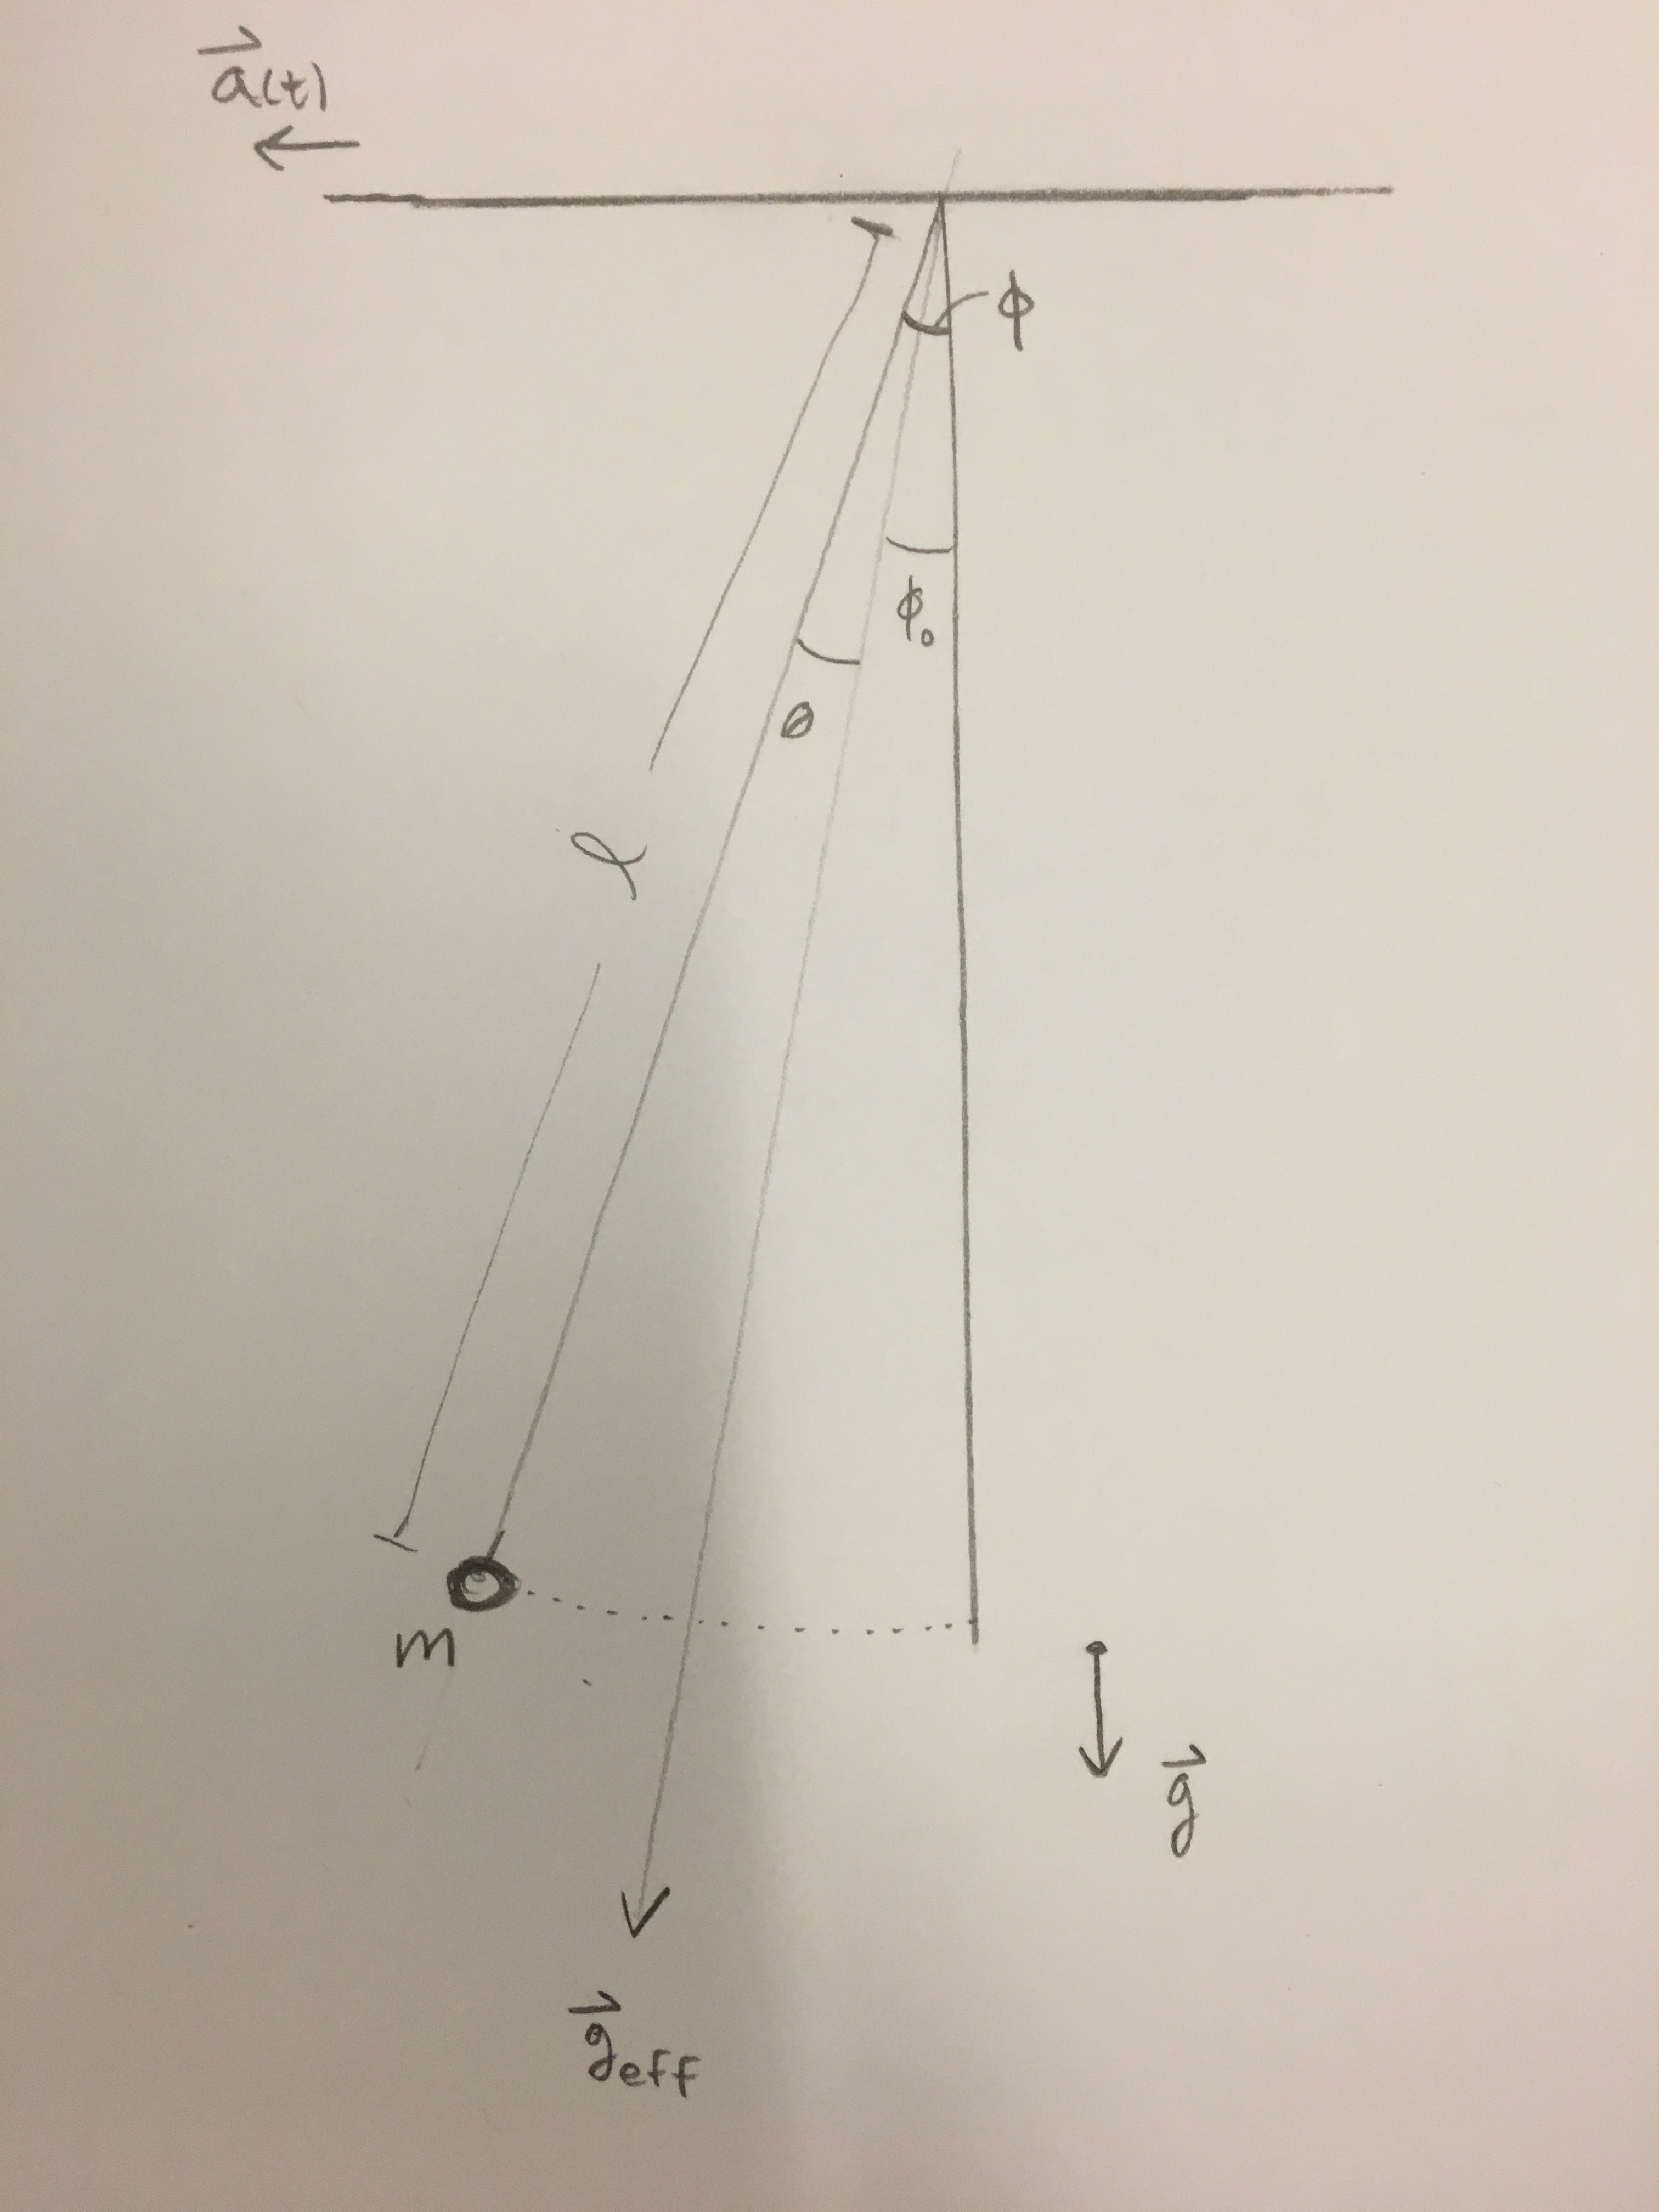
\includegraphics[width=.8\textwidth]{pendulum.jpg}
% 	\caption{Pendulum that starts at rest in an accelerating frame. If the acceleration is not constant then the apparent vertical, and thus $\phi_0$ will change with time}
% \end{figure}

\section{Results}

\subsection{Table}
Here are the results I got from theoretical and experimental calculations.
\begin{center}

	\begin{table}[H]
		\begin{tabular}{ | c | c | c | c | c | }
			\hline
			x  & p(x)                   & Frequency/N & F(x)                & Cumulative Frequency/N \\
			\hline\hline
			\hline
			0  & 0.36787944117144233    & 0.344       & 0.36787944117144233 & 0.344                  \\
			\hline

			1  & 0.36787944117144233    & 0.37        & 0.7357588823428847  & 0.714                  \\
			\hline

			2  & 0.18393972058572117    & 0.207       & 0.9196986029286058  & 0.9209999999999999     \\
			\hline

			3  & 0.06131324019524039    & 0.057       & 0.9810118431238462  & 0.978                  \\
			\hline

			4  & 0.015328310048810098   & 0.02        & 0.9963401531726562  & 0.998                  \\
			\hline

			5  & 0.0030656620097620196  & 0.002       & 0.9994058151824182  & 1.0                    \\
			\hline

			6  & 0.0005109436682936699  & 0.0         & 0.999916758850712   & 1.0                    \\
			\hline

			7  & 7.299195261338141e-05  & 0.0         & 0.9999897508033254  & 1.0                    \\
			\hline

			8  & 9.123994076672677e-06  & 0.0         & 0.9999988747974021  & 1.0                    \\
			\hline

			9  & 1.0137771196302974e-06 & 0.0         & 0.9999998885745217  & 1.0                    \\
			\hline

			10 & 1.0137771196302975e-07 & 0.0         & 0.9999999899522337  & 1.0                    \\
			\hline

			11 & 9.216155633002704e-09  & 0.0         & 0.9999999991683893  & 1.0                    \\
			\hline

			12 & 7.68012969416892e-10   & 0.0         & 0.9999999999364023  & 1.0                    \\
			\hline

			13 & 5.907792072437631e-11  & 0.0         & 0.9999999999954803  & 1.0                    \\
			\hline

			14 & 4.2198514803125934e-12 & 0.0         & 0.9999999999997002  & 1.0                    \\
			\hline

			15 & 2.8132343202083955e-13 & 0.0         & 0.9999999999999816  & 1.0                    \\
			\hline

			16 & 1.7582714501302472e-14 & 0.0         & 0.9999999999999991  & 1.0                    \\
			\hline

			17 & 1.0342773236060278e-15 & 0.0         & 1.0000000000000002  & 1.0                    \\
			\hline

			18 & 5.745985131144599e-17  & 0.0         & 1.0000000000000002  & 1.0                    \\
			\hline

			19 & 3.0242027006024205e-18 & 0.0         & 1.0000000000000002  & 1.0                    \\
			\hline

			20 & 1.5121013503012103e-19 & 0.0         & 1.0000000000000002  & 1.0                    \\
			\hline
		\end{tabular}
		\caption{\label{tab:data-table}Theoretical and Experimental Values Generated by Python Code}
	\end{table}
\end{center}


% \begin{figure}
% 	\centering
% 	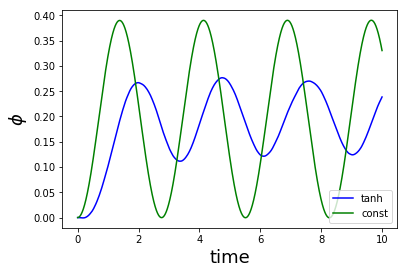
\includegraphics[width=.7\textwidth]{tanh_vs_const_1.png}
% 	\caption{Hyperbolic tangent acceleration vs immediate constant acceleration. The slow approach to the same asymptotic value of 2 meters per second per second induces a lag in the oscillation and also diminishes the amplitude of oscillation.}
% \end{figure}

Table \ref{tab:data-table} shows us that $p(x)$ and $Frequency/N$ values are apporximately similar. Same goes for $F(x)$ and $Cumulative Frequency/ N$. This is our expected result.

\subsection{Graphs}

\begin{figure}[H]
	\centering
	\begin{subfigure}{.5\textwidth}
		\centering
		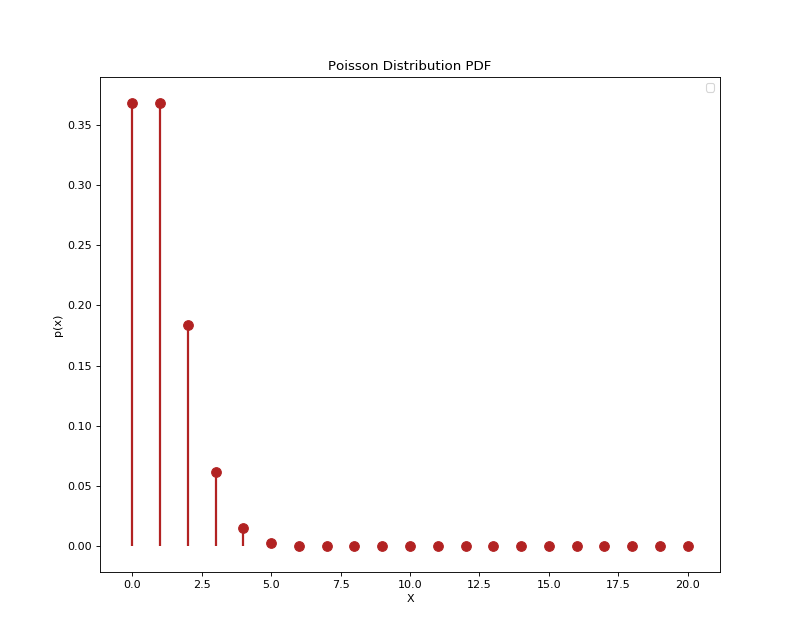
\includegraphics[scale=0.35]{Figures/pdf.png}
		\caption{p(x) vs x}
		\label{fig:px}
	\end{subfigure}%
	\begin{subfigure}{.5\textwidth}
		\centering
		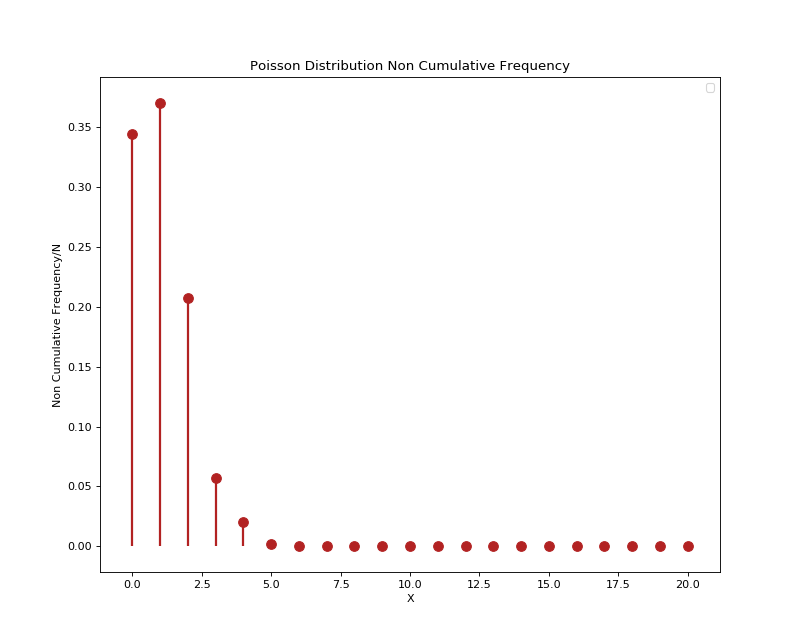
\includegraphics[scale=0.35]{Figures/noncumfreq.png}
		\caption{Frequency/N vs x}
		\label{fig:freq}
	\end{subfigure}
	\caption{PDF and Frequency Side by Side}
	\label{fig:test}
\end{figure}

\begin{figure}[H]
	\centering
	\begin{subfigure}{.5\textwidth}
		\centering
		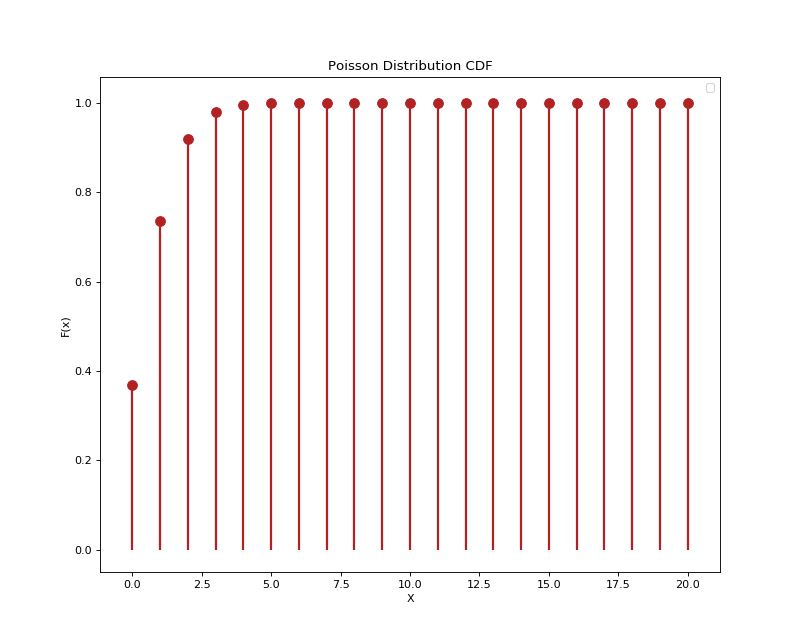
\includegraphics[scale=0.35]{Figures/cdf.png}
		\caption{F(x) vs x}
		\label{fig:fx}
	\end{subfigure}%
	\begin{subfigure}{.5\textwidth}
		\centering
		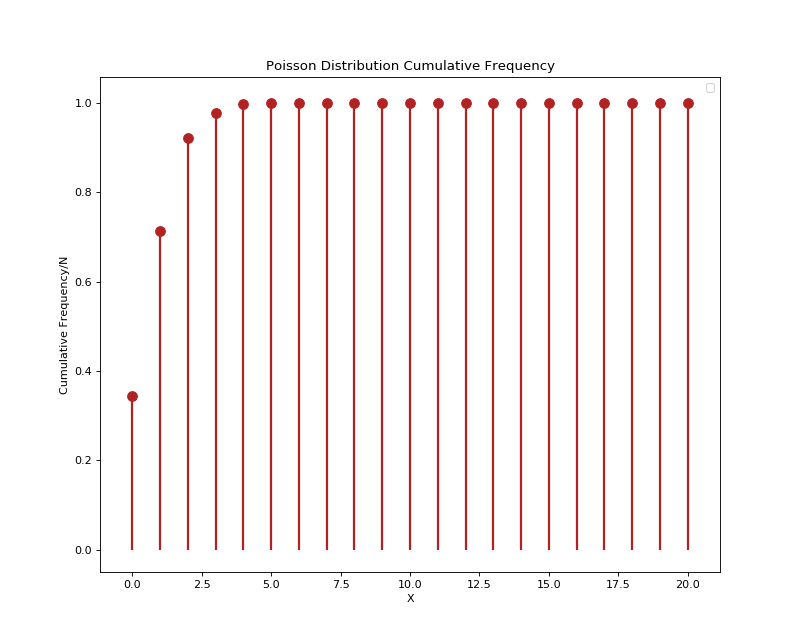
\includegraphics[scale=0.35]{Figures/cumfreq.png}
		\caption{Cumulative Frequency/N vs x}
		\label{fig:cumfreq}
	\end{subfigure}
	\caption{CDF and Cumulative Frequency Side by Side}
	\label{fig:test}
\end{figure}


\begin{figure}[H]
	\centering
	\begin{subfigure}{.5\textwidth}
		\centering
		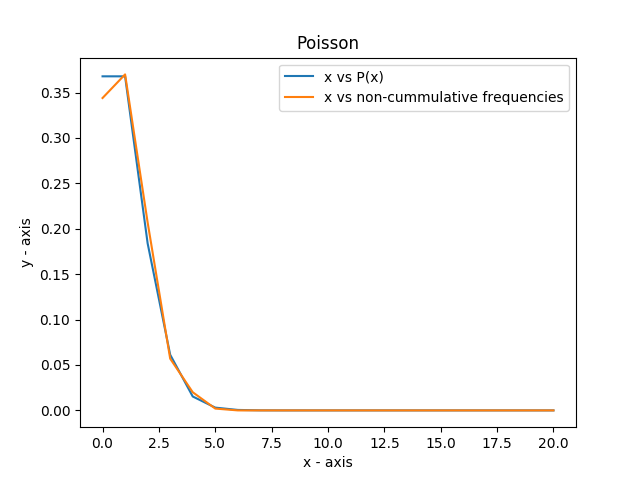
\includegraphics[scale=0.56]{Figures/pdf_noncum.png}
		\caption{Overlap of PDF and Frequency/N}
		\label{fig:fx}
	\end{subfigure}%
	\begin{subfigure}{.5\textwidth}
		\centering
		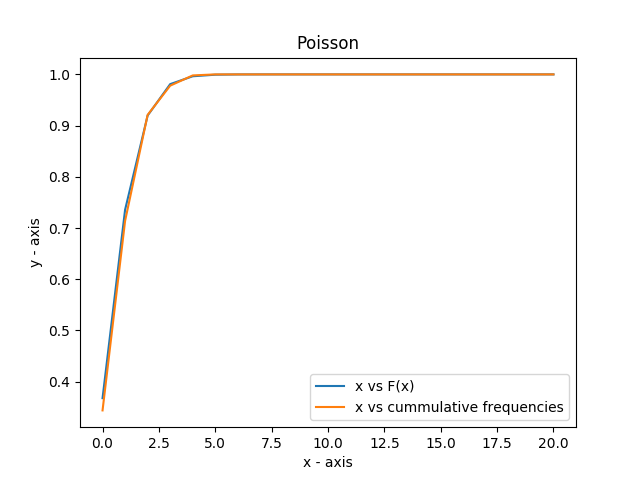
\includegraphics[scale=0.56]{Figures/cdf_cumfreq.png}
		\caption{Overlap of CDF and Cumulative Frequency}
		\label{fig:cumfreq}
	\end{subfigure}
	\caption{Similarities between graphs}
	\label{fig:overlap}
\end{figure}

\subsubsection{Observation}
From Graph \ref{fig:overlap} we can see that PDF almost overlaps with Frequency/N and CDF overlaps with Cumulative Frequency. That means, our experimental values are relevant with our theoretical values. 

\section{Conclusions}
Graph \ref{fig:overlap} actually shows us that our experimental and theoretical results are compatible to each other. So, we can generate N random variables using Poisson distribution. 

\end{document}
